\chapter{Conclusions}
\label{cha:evaluation}
\section{Summary of Achievements}
In summary, all project aims were fulfilled, except for the cost of service and ease of set-up aims, with attractiveness to open-source contributors is questionable. Other commercially available products cost less while providing similar or better functions, and the service is very challenging to self-deploy.

Core application - OpenFitCompanion was produced, an open-source alternative to health data aggregators and companions. Providing convenient access to all data in one place with an option to export it to a file, enabling further research such as comparing health tracking devices. Employing nudging mechanisms via daily and weekly reports, where users can effortlessly examine trends and progress towards their goals. Leveraging AI to create activity plans, selecting exercises to align with user's preferences and needs, with exercise reminders sent via push notifications. Lastly, enabling a natural language conversation about the user's health data, mimicking interaction with a personal trainer at a fraction of the cost. System structure was explained with the help of diagrams and key decisions justified. If AI is not used, the application is a strong alternative to similar systems like Google Fit. Although AI can provide useful insights, it also raises operating costs. Based on utility versus cost, it is hard to justify that our product is a better alternative.

Data analysis was performed to answer the research question concerning the equivalence of examined devices. Findings of exploration were presented: Bland-Altman plots, implications of initial findings and outlier protocol. Empirical difference percentages were calculated. An equivalence hypothesis testing problem was formulated, with the justification of statistical test used. Finally, results were interpreted, showing evidence of significant differences in the measurement of soft, moderate and intense activity seconds. Still, it is merely an interesting observation that warrants a more rigorous study involving more participants and a stricter data-gathering methodology. The artefact enables such studies to be performed easily and transparently.
\section{Critical Reflection}
\subsection{Product \& Investigation}
The cost was one of the driving factors to develop OpenFitCompanion so that users can enjoy features that commercial products lock behind an expensive subscription. Although there is one product that OpenFitCompanion beats on cost, it loses to all others. Another model or approach should have been tried. 

The project is not very attractive to potential open-source contributors due to the absence of tests and deployment automation. Tests allow collaborators to feel confident about system changes, preventing functional regression. At least for very critical portions, tests should have been created. For deployment, the project requires zipping lambda function folders and uploading them manually on the AWS web console one by one after every change. For a project that is cloud-centric, more attention should have been dedicated to automating the deployment pipeline.

User errors definitely took place during data collection for the analysis. There may be moderate errors, which were not detected using the outlier detection protocol. A more rigorous methodology for data collection should have been, such as journaling each day to sanity-check measurements from each device. 
\subsection{Personal}
I think the biggest difficulty was my lack of planning. Initially coming up with a very simplistic system that would not have enough complexity. My mindset was to first finish that and if I have time, then I expand to more features. After finishing that simple application, with the help of my supervisor and the wearables lab I got very interesting feature ideas such as incorporating a second device and using LLMs. However, the foundation of the system was too simple and could not support more complex features, so I had to re-engineer some parts of the system several times. I think I wasted a good chunk of time doing that, whereas I should have spent more time planning before implementation. Alternatively, I could have employed agile methodology and developed the system with high degrees of modularity and flexibility, therefore being able to cope with changing requirements more easily.

The previous point also led to me not having a clear schedule, mostly bouncing between working on different features with no deadlines set. Especially with LLM integration, I spent too much time designing prompts. This led me to have less time to polish other implementation aspects or work on the screencast and this report. I also tunnel-visioned on trying to make GPT4 work, whereas trying different models might have been more beneficial. 
\section{Further Work}
\subsection{Reducing AI inference cost}
\label{subsec:tryingOther}
As discussed in evaluation \ref{cha:evaluation}, the service does not compare well to other products mainly due to the cost of using GPT4 with Knowledge Retrieval (RAG), which is still an experimental feature at the time of writing. Maybe OpenAI improves the feature and allows more tuning or tinkering with file structure to fix the bug, however, other models should be examined. An obvious choice would be open-source models like LLAMA-2 or the recently released Grok-1, as on the surface they are free to use. However, using them locally, they are hard to set up and require commercial-level ML machines with a lot of VRAM. This is the reason they were not used initially. Cloud deployment is a more realistic prospect, with a rough estimate of using AWS Sagemaker to run LLAMA-2-13B on-demand costing 5£ per month. Still, open-source models perform worse than commercial ones like GPT4, whether utility is preserved while reducing costs needs to be confirmed with experimentation.

The other option is to use a newer commercial model. Claude 3 Sonnet, performs almost equally with GPT4, at a fraction of the cost. It is hard to classify which LLM benchmark reflects the nature of the task at hand, so the safe option is the "Mixed evaluations (BIG-Bench-Hard)" benchmark, which contains a mix of different tasks. Sonnet has 82.9\% performance against 83.1\% of GPT4 \cite{claude3Bench}, while having a cost of 3\$ per 1M tokens, which is 333\% less than GPT4.

Then health data can be put into context directly or using custom RAG. For example, sentence-transformers extract embeddings, then those are stored in a vector database such as Pinecone.

\subsection{Utilizing LLM vision}
The first idea is to use visual modality in LLMs for nutrition management. Nutrition is as important as exercise or sleep for improving the overall health. Existing commercial products mostly involve manually putting ingredients and it's quantity to estimate calories and macro-nutrients from the meal. Instead, this feature would involve just taking a picture of the meal, which is then processed by an LLM. MyfitnessPal has a similar feature where you scan the meal using the camera, however, from the demo and user feedback, it is apparent that it requires having very cleanly separated ingredients which are scanned one by one, struggling with meals where ingredients are slightly mixed. Preliminary investigation using Claude 3 Sonnet shows promise, it guesses the ingredients of a dish \ref{fig:sonnetV1} somewhat correctly, and then approximates the weight of each one \ref{fig:sonnetV2}.

The second idea is gym attendance accountability, requiring the user to take a selfie in the gym on designated days. This is like a friend keeping you accountable to a consistent gym schedule. The process would involve taking a fresh picture of the user with some distinct gym equipment in the background, then using LLM to verify if it is the same user and that they are in the gym. Camera API would be used rather than image upload, as users may upload old photos. Personalised encouraging messages could be sent on failure to verify, such as how many MET minutes the gym workout would contribute to reaching the weekly goal. 
\begin{figure}
    
    \centering
    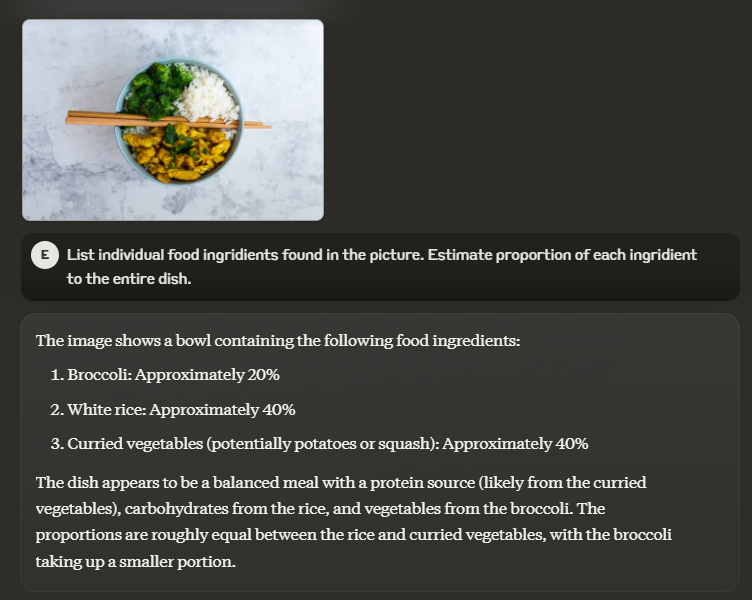
\includegraphics[width=1\textwidth,keepaspectratio]{../images/sonnet_vision.png}
    \caption{Claude 3 Sonnet identifies ingredients in a dish}
    \label{fig:sonnetV1}
    
\end{figure}
\begin{figure}
    
    \centering
    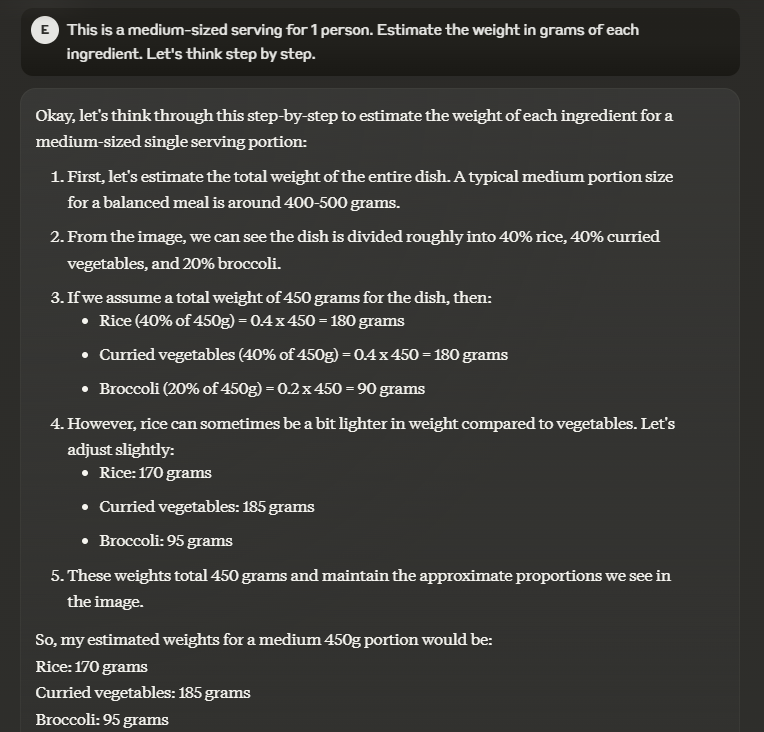
\includegraphics[width=1\textwidth,keepaspectratio]{../images/sonnet_vision_2.png}
    \caption{Claude 3 Sonnet approximates the weight of each ingredient of a dish}
    \label{fig:sonnetV2}
    
\end{figure}

\subsection{Avoiding Cloud vendor lock-in}
Cloud providers like AWS try to make it hard to switch to another provider. If AWS were to raise prices, it would be a laborious task to replicate the functionality on another cloud, like Azure. Then Azure could raise prices as well, requiring another rewrite or just accepting overpaying.

One option is OpenStack. It is a fundamentally different approach - it is an open-source, private cloud solution. Whereby you still have similar components of a typical cloud infrastructure but deployed on a particular machine. OpenStack is software which can run on any Linux machine, so it can be deployed on any physical machine or virtual machine (VM), with the latter probably being a more practical option for a non-technical user. Taking this option would make the project cloud provider independent, as migrating simply involves provisioning some VMs on another cloud. Notably, Mixtral provides a ready-to-deploy LLM via OpenStack, so this could tie in with earlier suggestion \ref{subsec:tryingOther}.
